%======================================================================
\section{The instrument and the regulatory framework}\label{sec:institutions}
%======================================================================

This section describes the features of AT1 bonds that the model must reproduce, the
regulatory rules behind them, and the three BNP Paribas bonds studied in the paper.
References to articles are to the Capital Requirements Regulation (CRR, Regulation (EU)
No 575/2013), the Capital Requirements Directive (CRD, Directive 2013/36/EU) and the
Bank Recovery and Resolution Directive (BRRD, Directive 2014/59/EU), as amended.

\subsection{Place in the capital structure}

A bank's own funds are layered. Common Equity Tier~1 (CET1) is ordinary share capital
and reserves; Additional Tier~1 (AT1) instruments complete Tier~1 capital, the
going-concern layer; Tier~2 instruments are gone-concern capital, subordinated debt
with an original maturity of at least five years. Below own funds, the bank's
loss-absorbing capacity in resolution (TLAC for global systemically important banks,
MREL for all banks) is completed by senior non-preferred debt, which ranks ahead of
Tier~2 but behind senior preferred debt and deposits.

In a liquidation or a resolution the creditor hierarchy determines the order in which
losses are absorbed: CET1 first, then AT1, then Tier~2, then senior non-preferred, then
senior preferred. For pricing purposes this ordering has a precise implication that we
use in Section~\ref{sec:t2}: every resolution event that imposes losses on Tier~2 has
already wiped out the AT1, while the converse is not true. AT1 holders are exposed to
all resolution events and, in addition, to events that hit AT1 alone.

\subsection{Eligibility and the perpetual call structure}

To count as AT1, an instrument must be perpetual, with no incentive to redeem (CRR
Art.~52). The issuer may call it no earlier than five years after issuance, and only
with the prior permission of the competent authority (Art.~77). Permission requires
that the instrument be replaced by own funds of equal or higher quality on terms that
are sustainable for the bank's income, or that the bank demonstrate that its own funds
would exceed its requirements by a margin the authority considers necessary (Art.~78).

The bonds studied here are callable only on their reset dates, every five years from
the first call. If not called, the coupon resets to the prevailing five-year US
Treasury constant-maturity yield plus the margin fixed at issuance. The fixed margin is
the source of extension risk: the issuer calls when it can refinance at a lower spread,
and does not call when spreads have widened, which is when investors would most like
their money back. Because the margin is fixed and the reference rate floats, the
economic call decision compares the reset margin with the issuer's new-issue AT1 spread
over the same benchmark; the level of rates cancels.

In practice, European issuers have called AT1s at the first opportunity in almost all
cases, partly for reputational reasons: a bank that does not call signals that its
funding is expensive. The best-known exception, Banco Santander's decision in early 2019
not to call a euro AT1, was widely reported precisely because it was rare. The model's
base call rule is purely economic; Section~\ref{sec:robust} adds a reputational
tolerance.

\subsection{Discretionary coupons and the Maximum Distributable Amount}

AT1 coupons are fully discretionary and non-cumulative: the issuer may cancel any
coupon at any time, cancelled coupons are lost, and cancellation is not an event of
default (CRR Art.~52(1)(l)). Coupons can only be paid out of distributable items.

In addition, coupons are mechanically restricted when the bank breaches its combined
buffer requirement (CRD Art.~141). Let the CET1 requirement be the sum of the Pillar~1
minimum ($4.5\%$ of risk-weighted assets), the CET1 part of the Pillar~2 requirement and
the combined buffer requirement (capital conservation, countercyclical, systemic risk
and G-SII/O-SII buffers). A bank whose CET1 ratio falls below this total may distribute
(dividends, variable remuneration and AT1 coupons together) at most the Maximum
Distributable Amount, a fraction of its interim and year-end profits that depends on
where the ratio sits inside the combined buffer:
\begin{center}
\begin{tabular}{lc}
\toprule
Position of CET1 inside the combined buffer & Maximum distributable fraction of profits \\
\midrule
top quartile & 0.6 \\
second quartile & 0.4 \\
third quartile & 0.2 \\
bottom quartile & 0 \\
\bottomrule
\end{tabular}
\end{center}
Two features of the rule matter for modelling. First, the MDA caps \emph{all}
distributions together; a bank inside the buffer chooses how to allocate the amount, and
would normally cut dividends, buy-backs and variable pay before cutting AT1 coupons,
which are small relative to profits and whose cancellation is costly for market access.
Applying the quartile factor to the coupon itself, as our model does, therefore
overstates the expected coupon loss. Second, analogous restrictions apply when the bank
breaches its leverage-ratio buffer (L-MDA) or its MREL requirement (M-MDA); for some
banks these bind before the CET1-based MDA.

\subsection{Loss absorption: trigger and point of non-viability}

Each AT1 contains a mechanical trigger: if the issuer's CET1 ratio falls below a
contractual level (at least $5.125\%$, CRR Art.~54), the instrument is converted into
ordinary shares or written down, permanently or temporarily. The bonds studied here
convert into shares at the higher of the prevailing market price and a floor price set
at issuance, so that the conversion ratio is capped.

Independently of the trigger, the resolution authority must write down or convert
capital instruments when the bank reaches the point of non-viability (BRRD Art.~59):
when the institution is failing or likely to fail and no alternative measure would
prevent its failure, or when public support is required. The write-down follows the
creditor hierarchy (BRRD Art.~48): CET1 first, then AT1, then Tier~2. A PONV write-down
can therefore occur while the CET1 ratio is far above the trigger. The Credit Suisse
case of March 2023, decided under Swiss law, wrote AT1 holders down to zero while
shareholders retained value; the EU authorities' joint statement of 20 March 2023
stated that in the EU, losses would continue to be absorbed by CET1 first and AT1 only
after CET1 had been fully used.

For pricing, this means two things. First, the PONV event is the dominant risk for a
well-capitalised issuer: the trigger is far away, but the regulator's decision is not
tied to it. Second, in the EU the PONV event that hits AT1 is, in most scenarios, the
same event that hits Tier~2. AT1 holders lose everything, Tier~2 holders lose part of
their claim. The AT1-specific part of the risk is the probability that AT1 is written
down while Tier~2 is not, together with the risk premia that investors attach to the
equity-like features of the instrument.

\subsection{The BNP Paribas bonds}

BNP Paribas is a global systemically important bank headquartered in France, supervised
by the ECB and resolvable by the Single Resolution Board. Its CET1 ratio was $12.97\%$ at
30 June 2026 against a published CET1 requirement of $10.43\%$. The latest stack available
item by item, at 30 September 2025, consists of Pillar~1 ($4.5\%$), the CET1 part of
Pillar~2R ($1.14\%$), the capital conservation buffer ($2.5\%$), the G-SIB buffer
($1.5\%$), the countercyclical buffer ($0.73\%$) and the systemic-risk buffer ($0.14\%$),
which sum to the $10.51\%$ requirement published at that date. The model takes the
Pillar~1 and Pillar~2R floor of $5.64\%$ from that stack and sets the combined buffer so
that the total equals the latest published requirement, $10.43\%$, so that the $8$bp
difference is attributed to the buffers. Under the French O-SII framework the
bank's O-SII buffer rises by 25bp on 1 January 2027 and by a further 25bp on 1 January
2028, and the higher of the G-SIB and O-SII buffers applies; at constant capital these
step-ups reduce the cushion above the MDA threshold from $2.5$ to $2.0$ percentage
points.

Table~\ref{tab:bonds} lists the three USD AT1s and the three bonds used as the Tier~2
and senior anchor. The AT1s share the issuer, the trigger ($5.125\%$ of group CET1), the
loss-absorption mechanism (conversion into ordinary shares) and the reset reference
(five-year US Treasury CMT); they differ in coupon, first call date and reset margin.
The Tier~2 and senior non-preferred (SNP) notes are callable once, one year before
maturity or at a reset date, when they cease to count as Tier~2 or MREL; the market
prices these calls as certain. The Tier~2 2035NC34 is the anchor: its call in November
2034 falls inside the AT1 call window (December 2033 to April 2036).

\begin{table}[H]
\centering\small
\begin{tabular}{llccccc}
\toprule
Bond & ISIN (144A) & Rank & Coupon & Call & Maturity & Reset margin \\
\midrule
6.875\% NC33 & US05602XQR25 & AT1 & 6.875\% & 15-Dec-2033 & perpetual & UST5 + 285bp \\
7.20\% NC36 & US05602XQS08 & AT1 & 7.200\% & 17-Apr-2036 & perpetual & UST5 + 294bp \\
7.45\% NC35 & US05602XQQ42 & AT1 & 7.450\% & 27-Jun-2035 & perpetual & UST5 + 313bp \\
\midrule
T2 2035NC34 & US09659T2D24 & T2 & 5.906\% & 19-Nov-2034 & 19-Nov-2035 & SOFR + 192bp \\
T2 2035NC30 & US09659T2B67 & T2 & 2.588\% & 12-Aug-2030 & 12-Aug-2035 & UST5 + 205bp \\
SNP 2035NC34 & US09659W2X16 & SNP & 5.738\% & 20-Feb-2034 & 20-Feb-2035 & SOFR + 188bp \\
\bottomrule
\end{tabular}
\caption{Bonds used in the paper. AT1s: perpetual, callable on reset dates every five
years, trigger $5.125\%$ of group CET1, conversion into ordinary shares at the higher of
the market price and a floor (USD 61.12, 72.52 and 61.17 per share respectively). Tier~2
and SNP: single call, treated as certain. Sources: BNP Paribas term sheets and debt
issuance list.}
\label{tab:bonds}
\end{table}

Figure~\ref{fig:prices} shows the AT1 prices over the sample. The 7.45\% has traded
since June 2025, the 6.875\% since December 2025 and the 7.20\% since April 2026. All
three fell by six to seven points over 2026, most of it from rising Treasury yields;
in the four weeks to 25 September 2026 the ten-year Treasury rose 45bp and the spread of
the low-margin 6.875\% widened by a further 34bp, against 10--12bp for the other two.

\begin{figure}[H]
\centering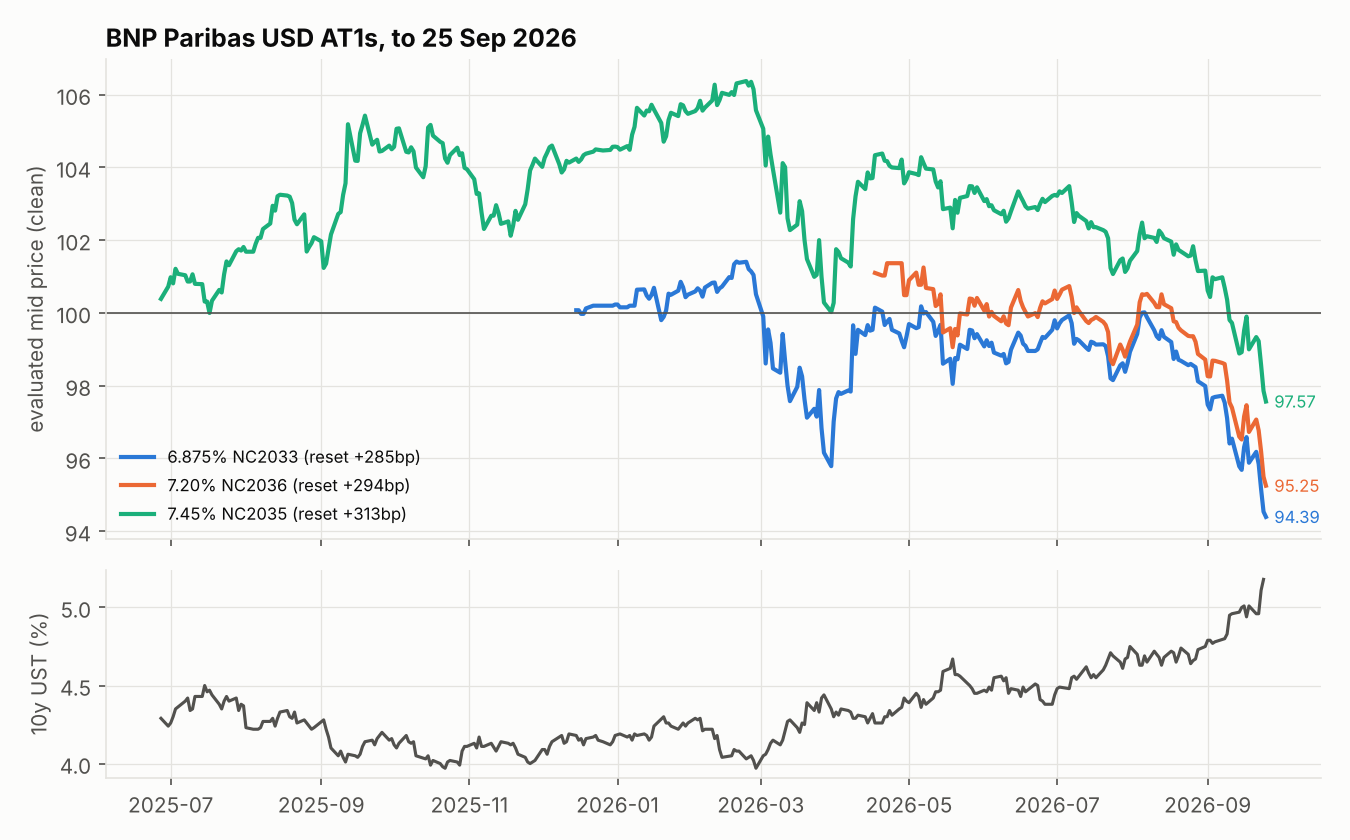
\includegraphics[width=0.92\textwidth]{bnp_at1_prices.png}
\caption{BNP Paribas USD AT1s: Capital IQ evaluated mid prices.}
\label{fig:prices}
\end{figure}